
\hypertarget{working_editor}{}
\section{Editor options}
\index{editor options}

The \textit{Editor options} window
(Figures \ref{fig:editor_display}, \ref{fig:editor_advanced} and \ref{fig:editor_keystrokes})
was adapted from the sources of the
\textit{SynEdit} component, mainly related to the general appearance and
standard options. The set of options available complement the
\textit{Application options} and allows high level of customization.


\hypertarget{working_editor_display}{}
\subsection{Display:}
\index{editor options!display}

\begin{figure}[h!]
  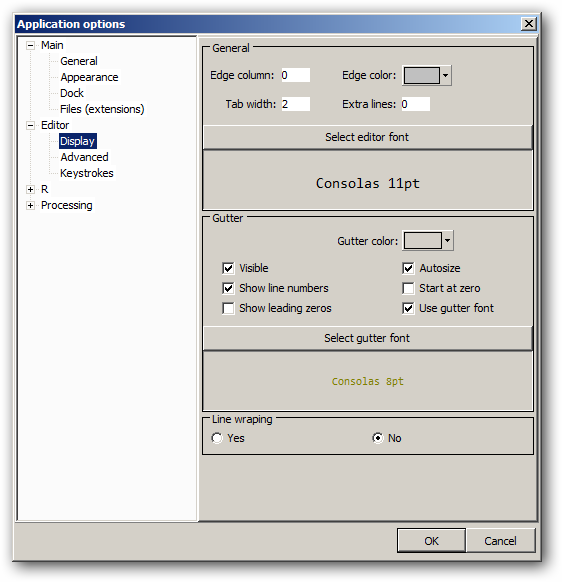
\includegraphics[scale=0.50]{./res/app_editor_display.png}~~
  \caption{Editor options: Display.}
  \label{fig:editor_display}
\end{figure}

\begin{table}
  \begin{footnotesize}
    \begin{tabularx}{\textwidth}{>{\hsize=0.3\hsize}X>{\hsize=0.7\hsize}X}\\
      \hline
      \textbf{Option} & \textbf{Description} \\
      \hline  %Display-----
      Edge column & Will be showed as a vertical line in the editor and the default is 80 characters.
      Set it to 0 or a negative value (-1) to make the edge column not visible \\
      Edge color & Choice of the edge color \\
      Tab width & Set the number of characters that will be inserted when typing the \textit{Tab} key \\
      Extra lines & Set the width which each single line will be displayed \\
      Font & Will open the Windows interface for choosing installed fonts \\
      \hline %Gutter-----
      Gutter color & Will open the Windows interface to choose a color \\
      Visible & Visibility option \\
      Autosize & Autosize option \\
      Show line number & Show line number option \\
      Start at zero & Start at zero option \\
      Show leading zeros & Show leading zeros option \\
      Use gutter font & Use gutter font option \\
      \hline
    \end{tabularx}
  \end{footnotesize}
  \caption{Display (Options/Editor).}
  \label{tab:editor_display}
\end{table}

Figure \ref{fig:editor_display} and
Table \ref{tab:editor_display}
show the main resources.

\hypertarget{working_editor_advanced}{}
\subsection{Advanced options}
\index{editor options!advanced}

\begin{figure}[h!]
  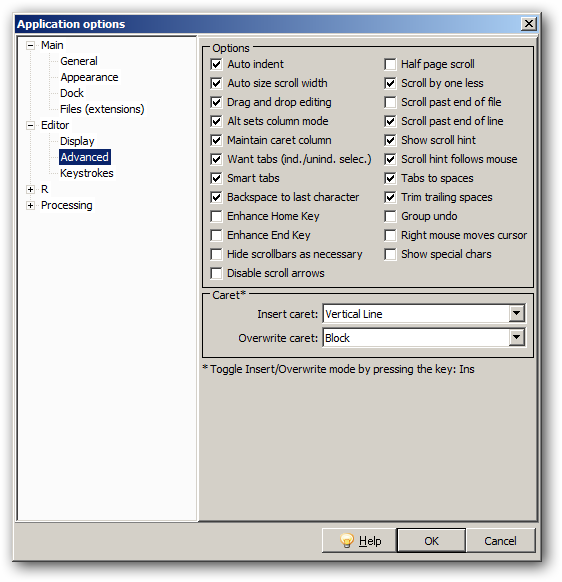
\includegraphics[scale=0.50]{./res/app_editor_advanced.png}~~
  \caption{Editor options: Advanced.}
  \label{fig:editor_advanced}
\end{figure}

\begin{table}
  \begin{footnotesize}
    \begin{tabularx}{\headwidth}{lX}\\
      \hline
      \textbf{Option} & \textbf{Description} \\
      \hline %Options-----
      Auto indent & Will indent the caret (position of the cursor in the current line) on new lines with the same amount of leading white space as the preceding line \\
      Auto size scroll width & Automatically resizes the MaxScrollWidth property when inserting text \\
      Drag and drop editing & Allows you to select a block of text and drag it within the document to another location \\
      Alt sets column mode & Holding down the $<$ALT$>$ key will put the selection mode into column format \\
      Maintain caret column & When moving through lines w/o cursor past EOL, keeps the X position of the cursor \\
      Want tabs & When active $<$TAB$>$ and $<$SHIFT$>$$<$TAB$>$ act as block indent, unindent when text is selected \\
      Smart tabs & When tabbing, the cursor will go to the next non-white space character of the previous line \\
      Smart tab delete & Similar to Smart Tabs, but when you delete characters \\
      Enhance home key & Enhances HOME key positioning, similar to visual studio \\
      Enhance end Key & Enhances END key positioning, similar to JDeveloper \\
      Hide scrollbars as necessary & If enabled, then the scrollbars will only show when necessary.
      If you have ScrollPastEOL, then the horizontal bar will always be there (it uses MaxLength instead) \\
      Disable scroll arrows & Disables the scroll bar arrow buttons when you can't scroll in that direction any more \\
      Half page scroll & When scrolling with page-up and page-down commands, only scroll a half page at a time \\
      Scroll by one less & Forces scrolling to be one less \\
      Scroll past end of file & Allows the cursor to go past the end of file marker \\
      Scroll past end of line & Allows the cursor to go past the last character into the white space at the end of a line \\
      Show scroll hint & Shows a hint of the visible line numbers when scrolling vertically \\
      Scroll hint follows mouse & The scroll hint follows the mouse when scrolling vertically \\
      Tabs to spaces & Converts a tab character to a specified number of space characters \\
      Trim trailing spaces & Spaces at the end of lines will be trimmed and not saved \\
      Group undo & When undoing/redoing actions, handle all continuous changes of the same kind in one call instead undoing/redoing
      each command separately \\
      Right mouse moves cursor & When clicking with the right mouse for a pop-up menu, move the cursor to that location \\
      Show special chars & Shows the special characters \\
      \hline %Caret-----
      Insert caret & A list with four options: Vertical line, Horizontal line, Half block and block \\
      Overwrite caret & A list with options: Vertical line, Horizontal line, Half block and block \\
      \hline
    \end{tabularx}
  \end{footnotesize}
  \caption{Display (Options/Editor).}
  \label{tab:editor_advanced}
\end{table}

Figure \ref{fig:editor_advanced} and
Table \ref{tab:editor_advanced}
show the main resources.


\hypertarget{working_editor_keystrokes}{}
\subsection{Keystrokes}
\index{editor options!keystrokes}

\begin{figure}[h!]
  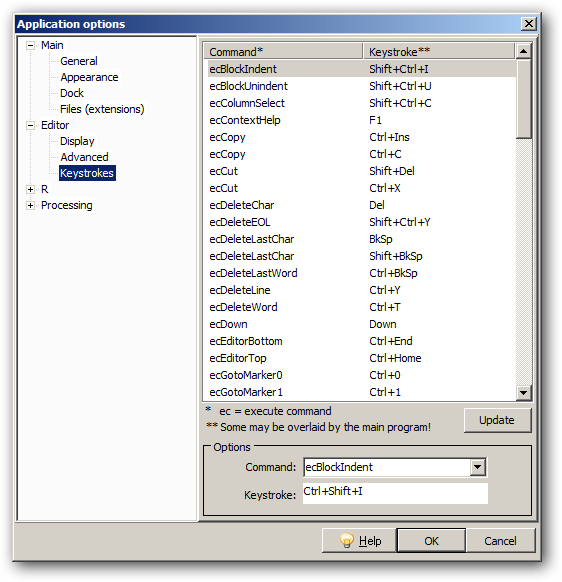
\includegraphics[scale=0.50]{./res/app_editor_keystrokes.png}\\
  \caption{Editor options: keystrokes.}
  \label{fig:editor_keystrokes}
\end{figure}

This interface
(Figure \ref{fig:editor_keystrokes})
allows to change the default SynEdit keystrokes.
It is possible to make new, edit or remove any ecAction (execute command action).
A set of user friendly keystrokes gives high productivity leading with
all instances of the main class \textit{SynEdit}: Editor, IO and Log.
